\documentclass{article}

\usepackage{fullpage, graphicx, multicol}
\usepackage[margin=0.1in, paperwidth=5.5in, paperheight=8.5in]{geometry}

\usepackage{tikz}
\usetikzlibrary{decorations.pathmorphing}

\usepackage[overlay, absolute]{textpos}

%%%%% Macros %%%%%%%%%%%%%%%%%%%%%%%%%%%%%%%%%%%%%%%%%%
\newcommand{\crossout}[1]{\raisebox{0mm}{%
    \tikz{\draw(0,0) node[anchor=west,inner sep=0,text depth=0.2mm](crossedWord){#1};
        \draw[decorate,decoration={random steps,amplitude=1pt},line width=3pt,opacity=0.6](crossedWord.west) -- (crossedWord.east);
      }}}

\newcommand{\person}[1]{\item #1}
\newcommand{\Xperson}[1]{\ifkeepOld \item \crossout{#1} \else\fi}
%%%%%%%%%%%%%%%%%%%%%%%%%%%%%%%%%%%%%%%%%%%%%%%%%%%%%%%

\newif\ifkeepOld
\renewcommand{\familydefault}{\sfdefault}  % default font
\def\labelitemi{--}                        % - instead of * for items.

%%%%%%%%%%%%%%%%%%%%%%%%%%%%%%%%%%%%%%%%%%%%%%%%%%%%%%%

%%%%% Keep old names? %%%%%%%%%%%%%%%%%%%%%%%%%%%%%%%%%
\keepOldtrue
%%%%%%%%%%%%%%%%%%%%%%%%%%%%%%%%%%%%%%%%%%%%%%%%%%%%%%%

\title{\Huge \textbf{Mathematically Structured Programming Group}}
\date{\vspace{-5ex}}

\begin{document}

\maketitle
\thispagestyle{empty} % remove page numbering

\begin{center}

\begin{multicols}{2}
\large
\begin{itemize}
  \Xperson{Robin Adams (Visitor)}
  \person{Guillaume Allais}
  \Xperson{Malin Altenm\"{u}ller}
  \person{Stevan Andjelkovic}
  \Xperson{Bob Atkey (RA)}
  \person{Simone Barlocco}
  \Xperson{Alwin Blok}
  \person{Peio Borthelle}
  \person{James Chapman (RA)}
  \person{Joseph Collins}
  \Xperson{Pierre-Evariste Dagand}
  \person{Kevin Dunne}
  \Xperson{Cl\'{e}ment Fumex}
  \person{Stuart Gale}
  \Xperson{Adam Gundry}
  \Xperson{Peter Hancock (RA)}
  \person{Alasdair Lambert}
  \Xperson{Sam Lindley (RA)}
  \Xperson{Ioan Luca}
  \Xperson{Lorenzo ``Mr. Baby'' Malatesta}
  \Xperson{Johannes Marti (RA)}
  \person{Fredrik Nordvall Forsberg (RA)}
  \Xperson{Federico Orsanigo}
  \person{Ben Price}
  \Xperson{Tim Revell}
  \Xperson{Denis Rochelle}
  \person{James Wood}
\end{itemize}
\end{multicols}
\vskip 3cm
\end{center}

{
\TPshowboxestrue
\TPMargin{6pt}
\textblockcolor{yellow!15}
\setlength{\TPboxrulesize}{2pt}
     \begin{textblock}{6.2}(7.5,12)
       \begin{center}
       {\Large \textbf{Combinatorics Group}}
     \end{center}
       \begin{itemize}
       \Xperson{Stuart Hannah}
       \person{Jason Smith (RA)}
       \end{itemize}
     \end{textblock}
}

{
%\TPshowboxestrue
%\TPMargin{6pt}
\textblockcolor{white}
%\setlength{\TPboxrulesize}{2pt}
     \begin{textblock}{3.5}(0.5,12)
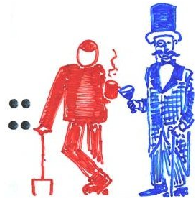
\includegraphics[scale=0.70]{semicolon.png}
     \end{textblock}
}

%\begin{tabular}{l r}
%\hskip 1cm
%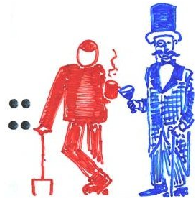
\includegraphics[scale=0.65]{semicolon.png} &
%\end{tabular}

\end{document}
